\chapter{Kürzeste Wege}

Wir betrachten einen Graph \( G = (V,E) \) mit Kantengewicht \( c: E \to \R \) und Anfangsknoten \( s \in V \).

Gesucht ist die Länge \( \mu(v) \) des \term{kürzesten Pfades}\index{Kürzester Pfad} von \( s \) nach \( v \) für alle \( v \in V \), wobei
\begin{equation*}
  \mu(v) \coloneqq \min\left \{ c(p) : p \text{ ist Pfad von \( s \) nach \( v \)} \right \}
\end{equation*}
und
\begin{equation*}
  c\left( \left\langle e_1,\dots,e_k \right\rangle \right) \coloneqq \sum_{i=1}^k c(e_i) \text{.}
\end{equation*}
Oft suchen wir auch eine ``geeignete'' Repräsentation des kürzesten Pfades.

\section{Allgemeine Definitionen}

Wir benutzen im Allgemeinen zwei Knotenarrays:
\begin{itemize}
  \item \( d[v] = \) aktuelle (= vorläufige) Distanz von \( s \) nach \( v \).

  \emph{Invariante}: \( d[v] \geq \mu(v) \).

  \item \( \text{parent}[v] = \) Vorgänger von \( v \) auf (vorläufigem) kürzesten Pfad von \( s \) nach \( v \).

  \emph{Invariante}: Dieser Pfad bezeugt \( d[v] \).
\end{itemize}
Initial ist
\begin{itemize}
  \item \( d[s] = 0 \), \( \text{parent}[s] = s \) und
  \item \( d[v] = \infty \), \( \text{parent}[v] = \perp \).
\end{itemize}
Kern ist das \emph{Relaxieren} der Kanten \( (u,v) \in E \):
\begin{pseudocode}
  \textbf{if} \( d[u] + c(u,v) < d[v] \) \textbf{then} \enskip \textcolor{gray}{// z.B. wenn \( d[v] \equiv \infty \)} \\
  \phantom{\enskip} \( d[v] \coloneqq d[u] + c(u,v) \) \\
  \phantom{\enskip} \( \text{parent}[v] \coloneqq u \)
\end{pseudocode}
Die oben genannten Invarianten werden dadurch nicht verletzt. \( d[v] \) kann sich also problemlos mehrmals ändern.

\section{Dijkstras Algorithmus}

Dijkstras Algorithmus ist der wohl einfachste Algorithmus, um dieses Problem zu lösen. In Pseudocode:

\begin{pseudocode}
  \textcolor{gray}{// \( d \) und parent initialisieren} \\
  \textcolor{gray}{// alle Knoten als ungescannt setzen} \\
  \textbf{while} \( \exists \) non-scanned node \( u \) with \( d[u] < \infty \) \textbf{do} \\
  \phantom{\enskip} \( u \coloneqq \) non-scanned node \( v \) with minimal \( d[v] \) \\
  \phantom{\enskip} relax all edges \( (u,v) \) out of \( u \) \\
  \phantom{\enskip} set \( u \) scanned
\end{pseudocode}

Ist \( v \in V \) von \( s \) aus erreichbar, so wird \( v \) irgendwann gescannt. Wird \( v \) gescannt, so ist \( \mu(v) = d[v] \).

Am Ende definiert \( d \) die optimalen Entfernungen und \code{parent} die zugehörigen Wege. Dieser Algorithmus wurde bereits in Algorithmen I ausführlich diskutiert.

\subsection{Analyse}

Es ist
\begin{equation*}
  T_{\text{Dijkstra}} = O(m*T_\text{decreaseKey}(n) + n*(T_\text{deleteMin}(n) + T_\text{insert}(n)))\text{.}
\end{equation*}
Nutzen wir also Fibonacci-Heaps, so kriegen wir
\begin{equation*}
  T_\text{DijkstraFib} = O(m+n\log n)\text{.}
\end{equation*}

\section{Monotone ganzzahlige Prioritätslisten}

Wir beobachten, dass Dijkstras Algorithmus die Prioritätsliste \emph{monoton} benutzt --- \code{insert} und \code{decreaseKey} benutzen nämlich Distanzen der Form \( d[u] + c(e) \). Die Werte nehmen also ständig zu.

Sind alle Kantengewichte \( \in [0,C] \), so gilt
\begin{equation*}
  \forall v \in V: d[v] \leq (n-1)C\text{.}
\end{equation*}
Ist insbesondere min der letzte Wert, der aus \( Q \) entfernt wurde, so sind in \( Q \) \emph{immer} nur Knoten mit Distanzen im Intervall \( [\min, \min+C] \).

\subsection{Bucket-Queue}

\begin{minipage}{.55\textwidth}
  Eine \term{Bucket-Queue}\index{Bucket-Queue} ist ein zyklisches Array \( B \) von \( C+1 \) doppelt verketteten Listen. Knoten der Distanz \( d[v] \) werden in \( B[d[v] \mod (C+1)] \) gespeichert.  
\end{minipage}
\hfill
\begin{minipage}{.5\textwidth}
  \begin{figure}[H]
    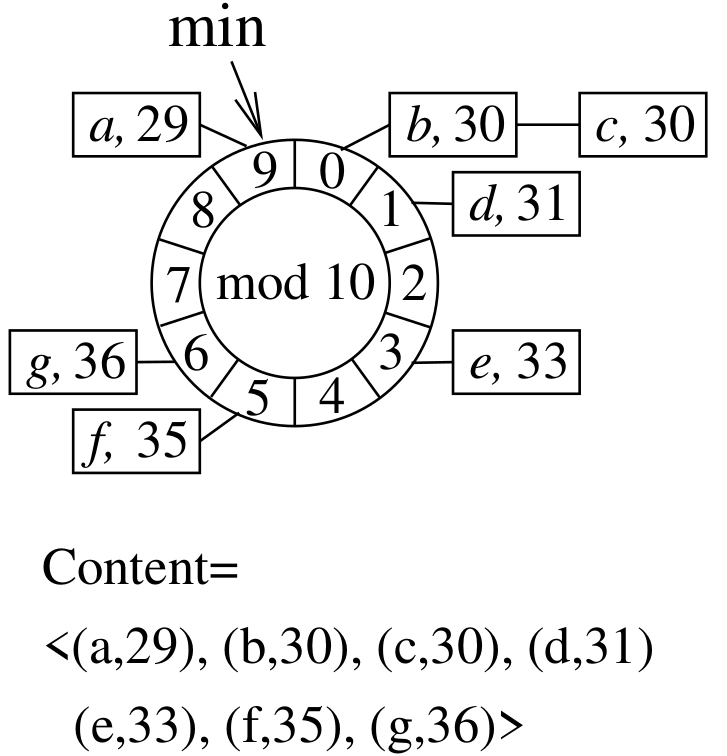
\includegraphics[width=.7\textwidth]{bucketQueue}
    \caption{Bucket-Queue mit \( C = 9 \)}
  \end{figure}
\end{minipage}

Folgende Operationen werden auf einer Bucket Queue implementiert:
\begin{itemize}
  \item \textbf{Initialisierung}: \( C+1 \) leere Listen werden angelegt, \( \min = 0 \).
  \item \textbf{\code{insert(v)}}: fügt \( v \) in \( B[d(v) \text{ mod } (C+1)] \) ein 
  
  \( \Rightarrow O(1) \)

  \item \textbf{\code{decreaseKey(v)}}: schiebt \( v \) von seiner Liste nach \( B[d(v) \text{ mod } (C+1)] \)

  \( \Rightarrow O(1) \)

  \item \textbf{\code{deleteMin}}: fängt bei \( B[\text{min mod } (C+1)] \) an; falls leer, \( \text{min} \coloneqq \text{min}+1 \), \( \circlearrowright \)
  
  \( \Rightarrow O(nC) \)
\end{itemize}

Mit Bucket-Queues kriegen wir also den Dijkstra-Algorithmus auf \( O(m+\text{maxPathLength}) \) gedrückt.

\subsection{Radix-Heaps}

Radix-Heaps sind eine Variante von Bucket Queues, die Buckets von \( -1 \) bis \( K \) für \( K = 1 + \lfloor \log C \rfloor \) benutzt. Wie vorhin schon betrachtet sei \( \min \) die zuletzt aus \( Q \) entfernte Distanz und somit
\begin{equation*}
  \forall v \in Q : d[v] \in [\min,\dots,\min+C]\text{.}
\end{equation*}

Wir betrachten die \emph{binäre Repräsentation} der möglichen Distanzen in \( Q \). Wir speichern \( v \) in Bucket \( B[i] \), falls sich \( d[v] \) und min zuerst an der \( i \)-ten Stelle unterscheiden (Ausnahmen: \( B[K] \) falls \( i > K \), \( B[-1] \) falls sie sich nicht unterscheiden).

Das definiert die \term{Most Significant Digit}\index{Most Significant Digit} (kurz MSD) --- das ist die Position der höchstwertigen Ziffer in der Binärdarstellung von \( a \) und \( b \), an der sich die beiden unterscheiden. \( \text{msd}(a,b) \) kann mit Maschinenbefehlen sehr schnell berechnet werden.

Wir nutzen folgende \emph{Radix-Heap-Invariante}:

\begin{center}
  \( v \) ist gespeichert in Bucket \( B[i] \), wo \( i = \min\left \{ \text{msd}(\min,d[v]),K \right \} \)
\end{center}

Wir können nun \code{deleteMin} folgendermaßen implementieren:

\begin{pseudocode}
  \textbf{\textsc{deleteMin}}\( () : \) Element \\
  \textbf{if} \( B[-1] = \varnothing \) \textbf{then} \\
  \phantom{\enskip} \( i \coloneqq \min\left \{ j \in 0\dots K : B[j] \neq \varnothing \right \} \) \\
  \phantom{\enskip} move \( \min B[i] \) to \( B[-1] \) and to min \\
  \phantom{\enskip} \textbf{foreach} \( e \in B[i] \) \textbf{do} \enskip{} \textcolor{gray}{// exactly here the invariant is violated!} \\
  \phantom{\enskip} \phantom{\enskip} move \( e \) to \( B[\min\left \{ \text{msd}(\min, d[v]), K \right \}] \) \\
  \textbf{return} \( B[-1]\text{.popFront}() \)
\end{pseudocode}

Die \code{deleteMin}-Laufzeit ist \( O(K) \), insgesamt lässt sich also die Laufzeit des Dijkstra-Algorithmus hierdurch auf \( O(m + n\log C) \) drücken.

\section{All-Pairs Shortest Paths}

Herausforderung in diesem Abschnitt ist es, nicht die Abstände zu einem festgelegten Startknoten zu berechnen, sondern zwischen allen Knotenpaaren \( (u,v) \in V^2 \) für \( G = (V,E) \). Zusätzlich erlauben wir negative Kantenkosten, allerdings keine negativen Kreise.

Wir werden zwei verschiedene Lösungen erhalten:

\begin{enumerate}
  \item \( n \) mal den \emph{Bellman-Ford-Algorithmus} ausführen

  \( \Rightarrow O(n^2m) \)

  \item \emph{Knotenpotentiale} verwenden

  \( \Rightarrow O(nm + n^2\log n) \)
\end{enumerate}

\subsection{Bellman-Ford-Algorithmus}

Der \term{Bellman-Ford-Algorithmus}\index{Bellman-Ford-Algorithmus} wurde bereits in Algorithmen I behandelt, deswegen hier nur eine kurze Wiederholung. Wie Dijkstras Algorithmus findet er den kürzesten Pfad zwischen einem festgelegten Startknoten und allen anderen Knoten des Graphen, unterstützt aber auch negative Kantengewichte.

\begin{enumerate}
  \item Distanzen initialisieren: \( d[s] = 0 \), \( d[v] = \infty \) für alle anderen Knoten
  \item Von \( s \) ausgehend alle Knoten des Graphen durchgehen und pro Knoten \( v \) die ausgehenden Kanten betrachten.
  \begin{itemize}
    \item Eintragen, ob \( v \) von \( s \) in \( < \infty \) erreicht werden kann.
    \item Ist \( d[v] + c(v,u) < d[u] \) für einen Nachbar von \( v \)? Wenn ja, \( d[u] \) aktualisieren.
  \end{itemize}
\end{enumerate}

Der zweite Schritt wird maximal \( \left\vert V \right\vert - 1 \) mal wiederholt. Sollte sich schon davor bei einem Durchgang nichts mehr ändern, so kann man aufhören.

Die Laufzeit des Bellman-Ford-Algorithmus ist \( O(nm) \), nutzt man ihn als Basis für All-Pairs Shortest Paths kriegt man also \( O(n * nm) = O(n^2m) \).

\subsection{Knotenpotentiale}

Jeder Knoten erhält ein Potential \( \text{pot}(v) \). Mit diesen Knotenpotentialen lassen sich die \term{reduzierten Kosten} \( \overline{c}(e) \) für eine Kante \( e = (u,v) \in E \) als
\begin{equation*}
  \overline{c}(e) = \text{pot}(u) + c(e) - \text{pot}(v)
\end{equation*}
definieren.

Ist \( p \) ein Pfad von \( u \) nach \( v \) mit Kosten \( c(p) \), dann ist
\begin{equation*}
  \overline{c}(p) = \text{pot}(u) + c(p) - \text{pot}(v)\text{.}
\end{equation*}

Ist \( p' \) ein anderer \( u \)-\( v \)-Pfad, dann gilt
\begin{equation*}
  c(p) \leq c(p') \Leftrightarrow \overline{c}(p) \leq \overline{c}(p')\text{.}
\end{equation*}

Wir berechnen die gewünschten Informationen nun so:
\begin{enumerate}
  \item Wir fügen einen \emph{Hilfsknoten} \( s \) zu \( G \) hinzu.
  \item Wir fügen \( (s,v) \) für alle \( v \in V \setminus \left \{ s \right \} \) mit Kosten \( 0 \) hinzu.
  \item Berechne die kürzesten Pfade von \( s \) aus mit Bellman-Ford.
  \item Definiere \( \text{pot}(v) \coloneqq \mu(v) \) für alle \( v \in V \).

  Die reduzierten Kosten sind jetzt alle nicht-negativ, also können wir Dijkstra benutzen und ggf. \( s \) wieder entfernen.
  \item Für eine beliebige Kante \( (u,v) \in E \) gilt
  \begin{equation*}
    \mu(u) + c(e) \geq \mu(v) \enskip \text{und deshalb} \enskip \overline{c}(e) = \mu(u) + c(e) - \mu(v) \geq 0\text{.}
  \end{equation*}
\end{enumerate}

\begin{pseudocode}
  neuen Knoten \( s \) und alle Kanten \( s,v \) hinzufügen \enskip{} \textcolor{gray}{// \( O(n) \)} \\
  \( \text{pot} \coloneqq \mu \coloneqq \textsc{BellmanFordSSSP}(s,c) \) \enskip{} \textcolor{gray}{// \( O(nm) \)} \\
  \textbf{foreach} \( x \in V \) \textbf{do} \\
  \phantom{\enskip} \( \overline{\mu}(x,\cdot) \coloneqq \textsc{DijkstraSSSP}(x,\overline{c}) \) \\
  \ \\
  \textcolor{gray}{// zurück zur ursprünglichen Kostenfunktion} \\
  \textbf{foreach} \( e = (v,w) \in V^2 \) \textbf{do} \enskip \textcolor{gray}{// \( O(n^2) \)} \\
  \phantom{\enskip} \( \mu(v,w) \coloneqq \overline{\mu}(v,w) + \text{pot}(w) - \text{pot}(v) \)
\end{pseudocode}

Die Gesamtlaufzeit beträgt also \( O(nm + n^2\log n) \).

\section{Distanz zu Zielknoten}

Wir haben bisher zwei Fälle diskutiert:
\begin{enumerate}
  \item Abstände aller Knoten zu einem Startknoten \( s \)
  \item Abstände zwischen allen Knotenpaaren \( \left \{ u,v \right \} \in V^2 \)
\end{enumerate}

Als nächstes schauen wir uns an, wie man den kürzesten Pfad zwischen einem Startknoten \( s \) und einem Zielknoten \( t \) ermittelt.

\subsection{Trick 0 --- Dijkstra abbrechen}

Am einfachsten ist es, einfach Dijkstra abzubrechen, wenn \( t \) aus \( Q \) entfernt wird. Das spart ``im Schnitt'' die Hälfte des Scans.

\subsection{Bidirektionale Suche}

Idee ist hier, abwechselnd von \( s \) und \( t \) aus zu suchen. Von \( s \) aus sucht man auf \( G = (V,E) \), von \( t \) aus auf dem zugehörigen \emph{Rückwärtsgraphen} \( G^r = (V,E^r) \).

Die vorläufige kürzeste Distanz wird in jedem Schritt gespeichert:
\begin{equation*}
  d[s,t] = \min\left \{ d[s,t],d_\text{forward}[u] + d_\text{backward}[u] \right \}
\end{equation*}

Abgebrochen wird, wenn die Suche einen Knoten scannt, der in die andere Richtung bereits gescannt wurde.

\subsection{\( A^\ast \)-Suche}

Idee der \( A^\ast \)-Suche ist es, ``in die Richtung'' des Ziels zu suchen. Dazu benötigen wir eine Funktion \( f(v) \), die für alle \( v \in V \) die eigentliche Funktion \( \mu(v,t) \) schätzen kann.

Anschließend können wir \( \text{pot}(v) = f(v) \) setzen und \( \overline{c}(u,v) = c(u,v) + f(v) - f(u) \).

\( f(v) \) muss diese Eigenschaften haben:
\begin{itemize}
  \item \textbf{Konsistenz}: \( c(e) + f(v) \geq f(u) \) (\( \forall e = (u,v) \)). 

  Die reduzierten Kosten dürfen also nicht negativ sein.

  \item \( f(v) \leq \mu(v,t) \) (\( \forall v \in V \)).

  Dann ist \( f(t) = 0 \) und wir können aufhören wenn \( t \) aus \( Q \) entfernt wird.
\end{itemize}

Ist \( p \) ein beliebiger Pfad von \( s \) nach \( t \), so ist \( d[t] \leq c(p) \) (alle Kanten auf \( p \) seien relaxiert). Wie finden wir jetzt aber so eine Funktion \( f(v) \)?

Wir benötigen eine Heuristik für \( f(v) \).

\begin{itemize}
  \item Betrachtet man eine Strecke im Straßennetzwerk, so kann \( f(v) \) beispielsweise der euklidische Abstand \( \left\Vert v - t \right\Vert_2 \) sein. Damit erhält man eine deutliche, aber keine überragende Beschleunigung.
  \item \term{Landmarks}\index{Landmarks} sind deutlich geeigneter, benötigen allerdings Vorberechnung.

  Man wähle eine \emph{Landmarkmenge} \( L \). Berechne und speichere \( \mu(v,l) \) für alle \( l \in L, v \in V \).

  Während einer Query suche man jetzt ein Landmark \( l \in L \) ``hinter'' dem Ziel und benutze die untere Schranke
  \begin{equation*}
    f_l(v) = \mu(v,l) - \mu(t,l)
  \end{equation*}
  \emph{Vorteile} sind, dass Landmarks konzeptuell einfach sind, eine erhebliche Beschleunigung bringen (um den Faktor 20) und mit anderen Techniken kombinierbar sind.

  \emph{Allerdings} ist die Landmarkauswahl schwierig und der Platzverbrauch sehr groß (besonders für große \( V \)).
\end{itemize}